\chapter{Square Circle usage during the Boer War}

\begin{figure*}
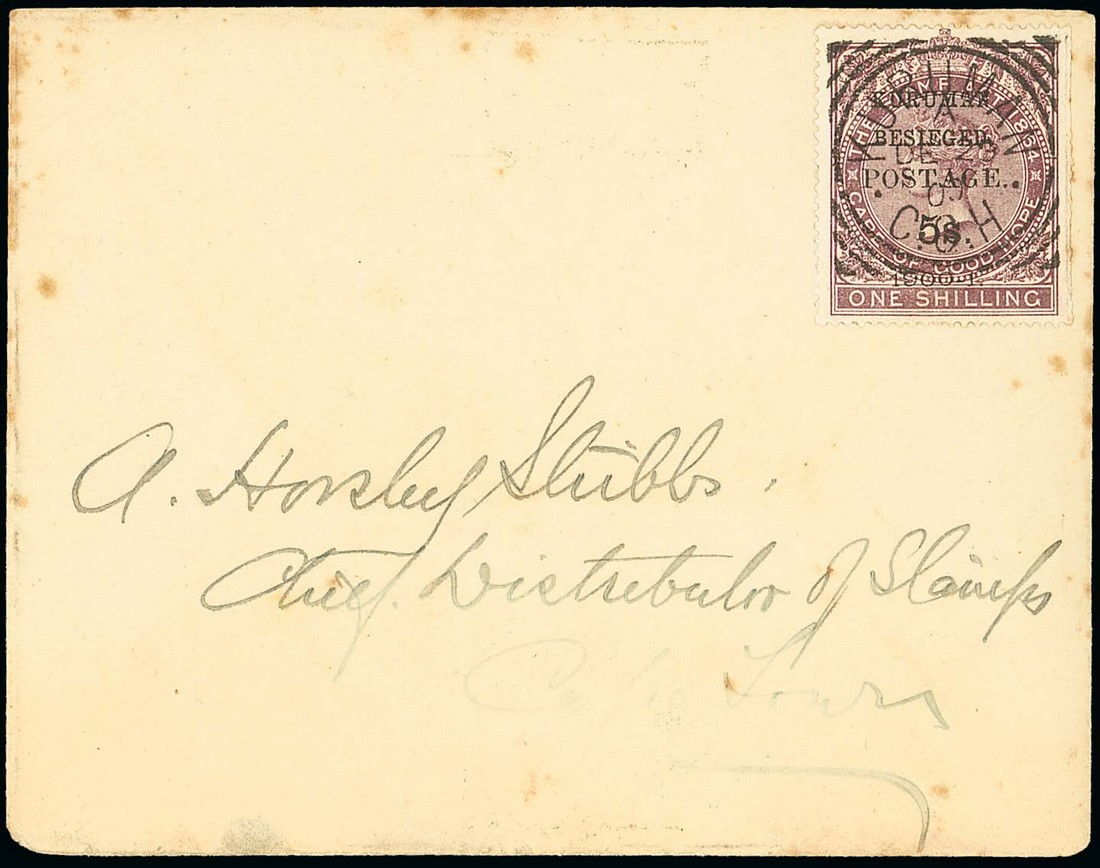
\includegraphics[width=1.0\textwidth]{../cape-of-good-hope/14018_144_1.jpg}
\caption{Lot: 144 (x) Kuruman
The town was besieged for the first time from 13 November 1899 to 1 January 1900 when it surrendered to Boer forces. General Warren re-occupied the town from 24 June 1900
The Stamp Surcharges
The following group of stamps were prepared for use but owing to the relief of the town within a week their use became unnecessary
Surcharged on Revenue Stamps Overprinted "postage"
5/- on 1/- purple, neatly cancelled by 29 December squared-circle datestamp and affixed to envelope (some foxing) addressed to Horsley Stubbs "Chief Distributor of Stamps" at Cape Town; perfs. largely trimmed at right. Estimate  \pound500 to  \pound600}
\end{figure*}

\begin{figure*}
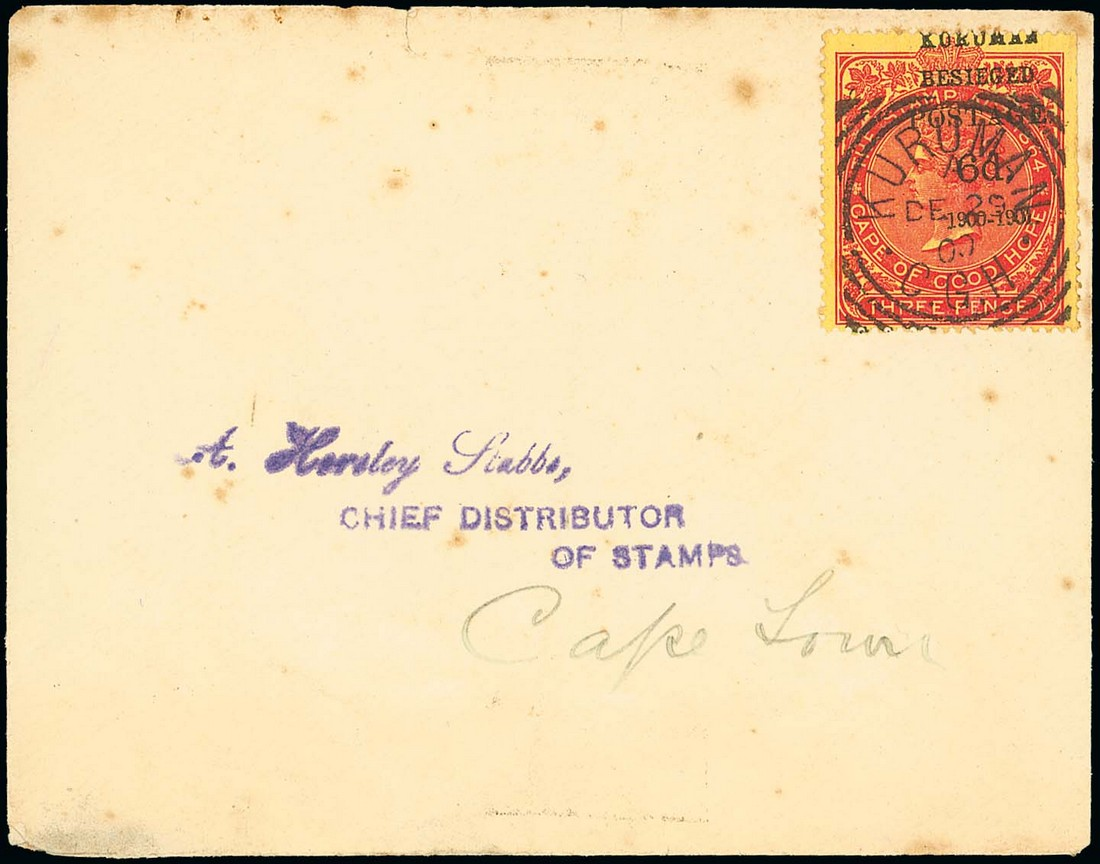
\includegraphics[width=1.0\textwidth]{../cape-of-good-hope/14018_143_1.jpg}
\caption{Lot: 143 (x) Kuruman
The town was besieged for the first time from 13 November 1899 to 1 January 1900 when it surrendered to Boer forces. General Warren re-occupied the town from 24 June 1900
The Stamp Surcharges
The following group of stamps were prepared for use but owing to the relief of the town within a week their use became unnecessary
Surcharged on Revenue Stamps Overprinted "postage"
6d. on 3d. red on yellow with small "1900-01", neatly cancelled by 29 December squared-circle datestamp and affixed to envelope (some foxing) addressed to Horsley Stubbs "Chief Distributor of Stamps" at Cape Town; believed to be the sole 6d. on 3d. value recorded on cover. Photo 
Estimate  \pound500 to  \pound600}
\end{figure*}